\usepackage{hyperref}

\appendix
\chapter{Supplementary material}
\section{Axelrod model: phase diagrams}
In addition to what is presented in the main section of the report, we also show how the critical value $q_c$ varies with $F$ for a given network topology. To this end, we repeated the same simulations as before, varying the value of $F$ at each run. The network parameters and sizes were kept fixed, and each simulation was run once for $2 \times 10^7$ iterations. The goal was to reproduce a phase diagram of the Axelrod model for a given topology. Due to computational constraints, we could not explore higher values of $F$, although doing so would provide more complete results.

\begin{figure}[hbtp]
    \centering
    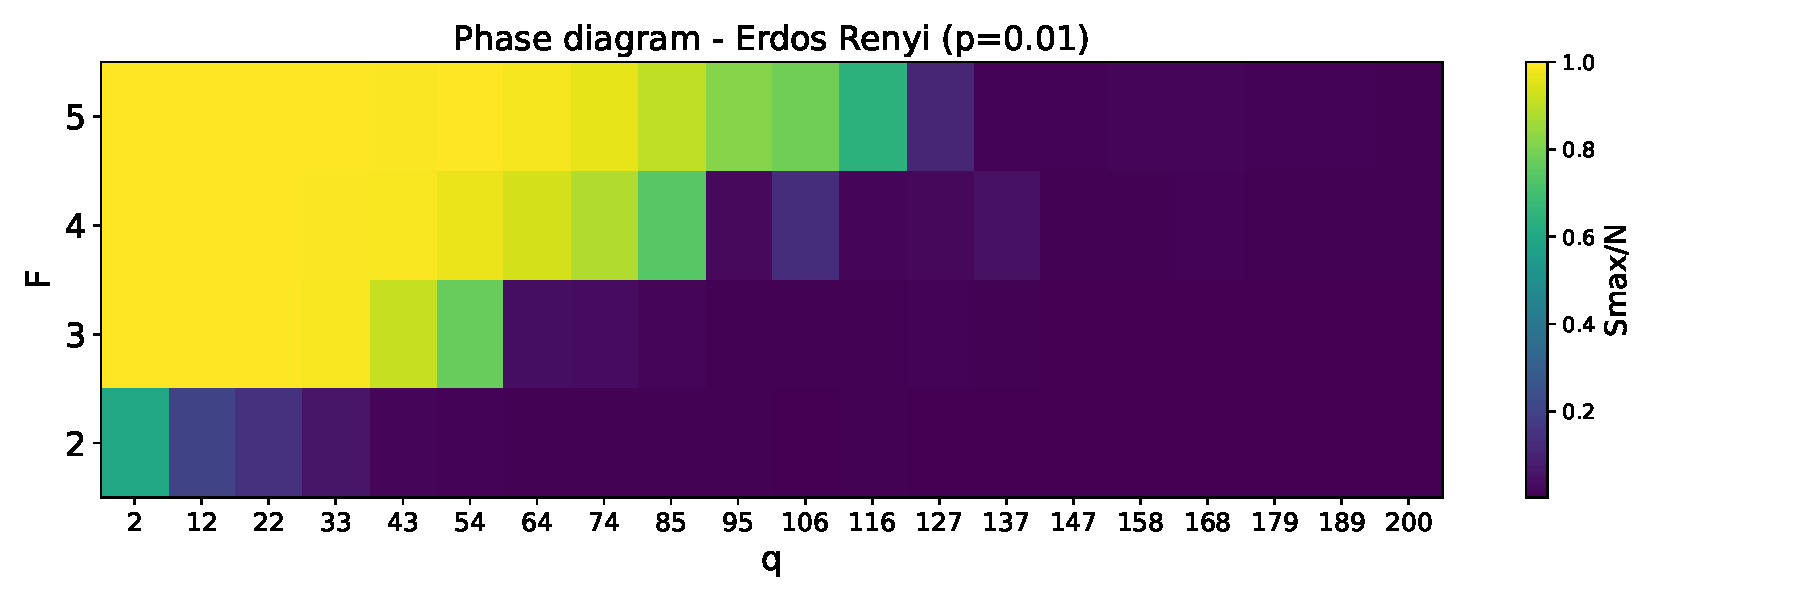
\includegraphics[width=0.75\linewidth]{task30_plots/phase_diagram_ER.pdf}
    \end{figure}

\begin{figure}[hbtp]
    \centering
    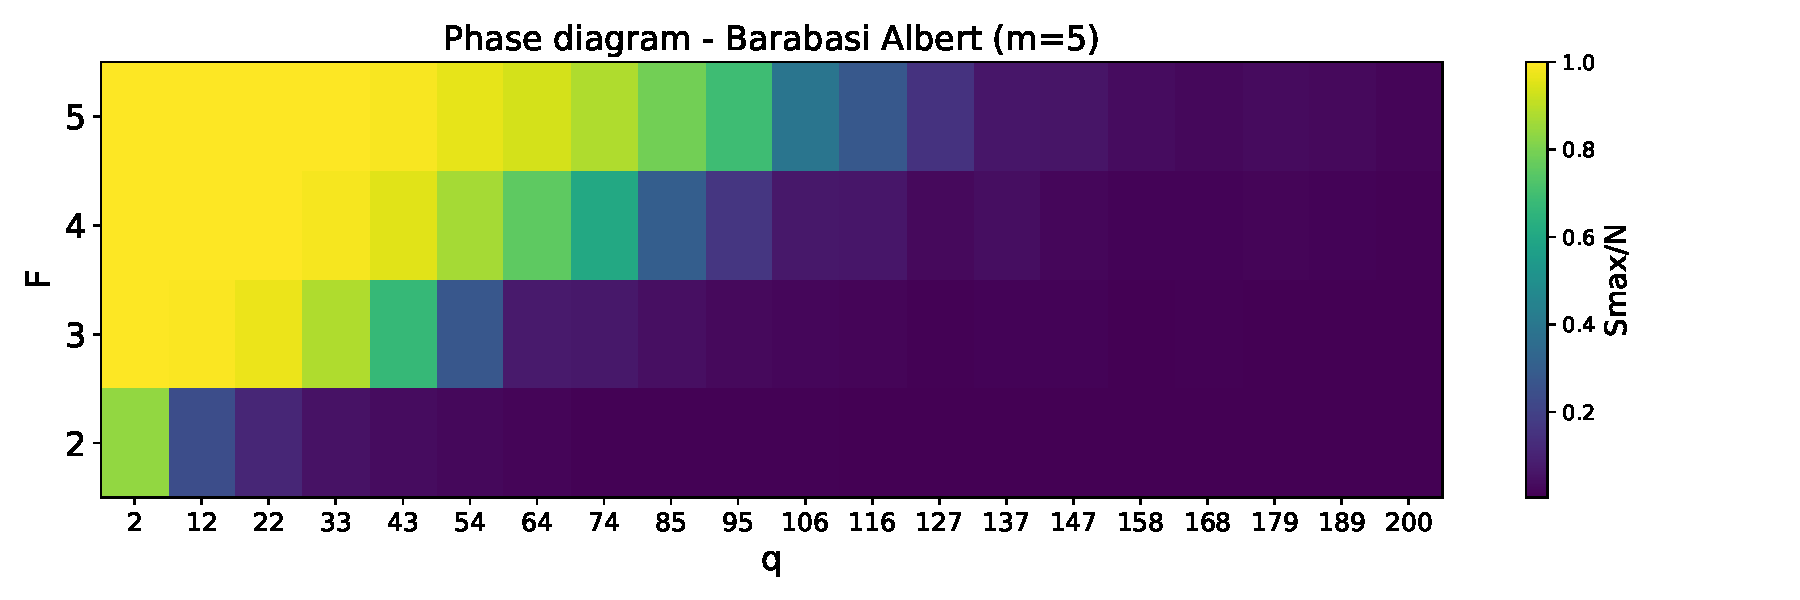
\includegraphics[width=0.75\linewidth]{task30_plots/phase_diagram_BA.pdf}
\end{figure}

\begin{figure}[hbtp]
    \centering
    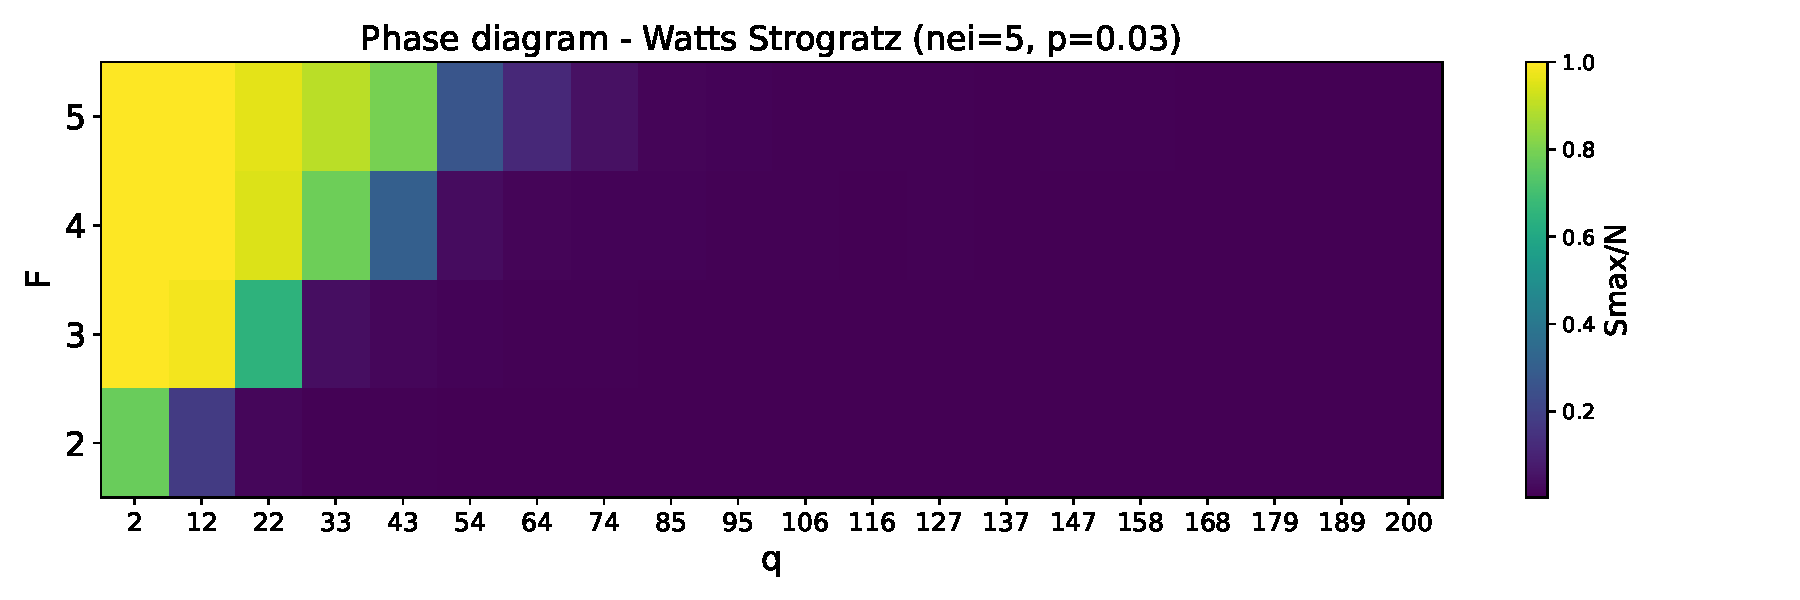
\includegraphics[width=0.75\linewidth]{task30_plots/phase_diagram_WS.pdf}
\end{figure}

In addition to the observations reported in the main section, the phase diagrams show that increasing the value of $F$ also increases $q_c$, as well as the number of iterations required for the system to reach an absorbing state.
This behavior reflects the fact that higher cultural complexity (larger $F$) increases the number of possible configurations, thus raising the threshold $q_c$ and slowing down convergence to consensus or polarization.

\section{Axelrod model: real network application}
In this section, we perform a further analysis using a real network, namely the "B.F. Maier's FB friends network," available at this \href{https://github.com/benmaier/BFMaierFBnetwork/blob/master}{GitHub repository} \cite{Maier2017}. The dataset consists of an anonymized Facebook friendship network collected in fall 2014. Nodes represent Facebook profiles, and edges represent friendships between them. The node corresponding to the profile owner, which was connected to every other node, has been removed.

Some basic network statistics are as follows:
\begin{itemize}
    \item Undirected: True
    \item Number of nodes: $N = 362$
    \item Number of edges: $1988$
    \item Mean degree: $10.98$
    \item Connected components: $20$
    \item Nodes in largest component: $329$
    \item Global clustering coefficient $C = 0.51$
    \item Average path length = $3.58$
\end{itemize}

We also plotted the degree distribution, shown in Fig.~\ref{fig:Maier_degree_distribution}.

\begin{figure}[hbtp]
    \centering
    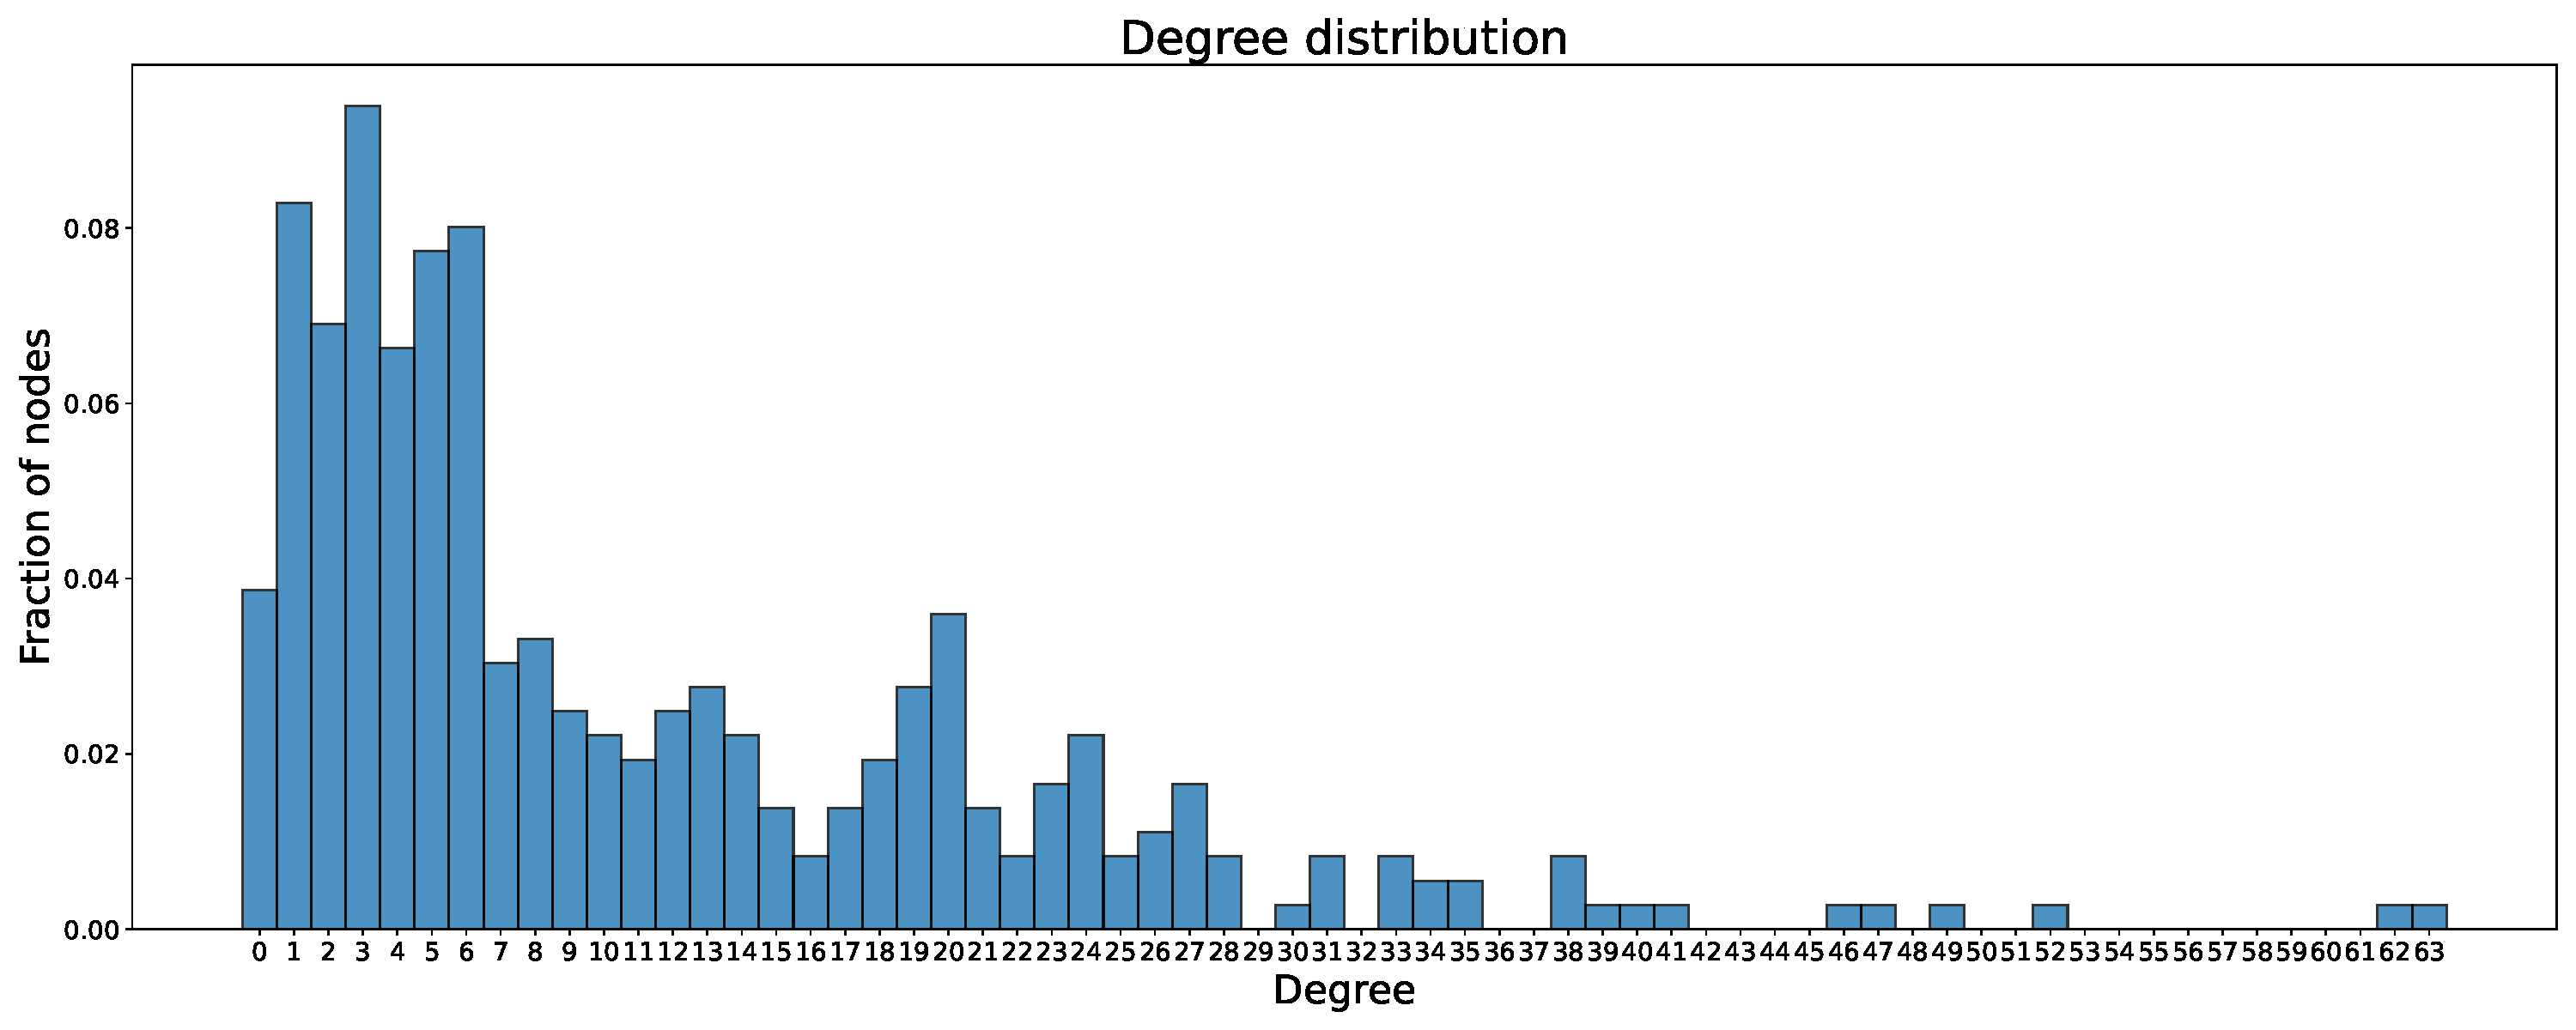
\includegraphics[width=0.8\linewidth]{task30_plots/Maier_degrees.pdf}
    \caption{Degree distribution of the B.F. Maier FB friends network.}
    \label{fig:Maier_degree_distribution}
\end{figure}

We performed the same analysis as before and produced the same type of phase transition plot, comparing the real network with synthetic networks of the same size. The parameters of the synthetic networks were chosen to match the average degree of the real network ($p = 0.03$ for Erdős-Rényi, $m = 5$ for Barabási-Albert, and $nei = 5$, $p_{ws} = 0.03$ for Watts-Strogatz), in order to ensure comparability across topologies.

\begin{figure}[hbtp]
    \centering
    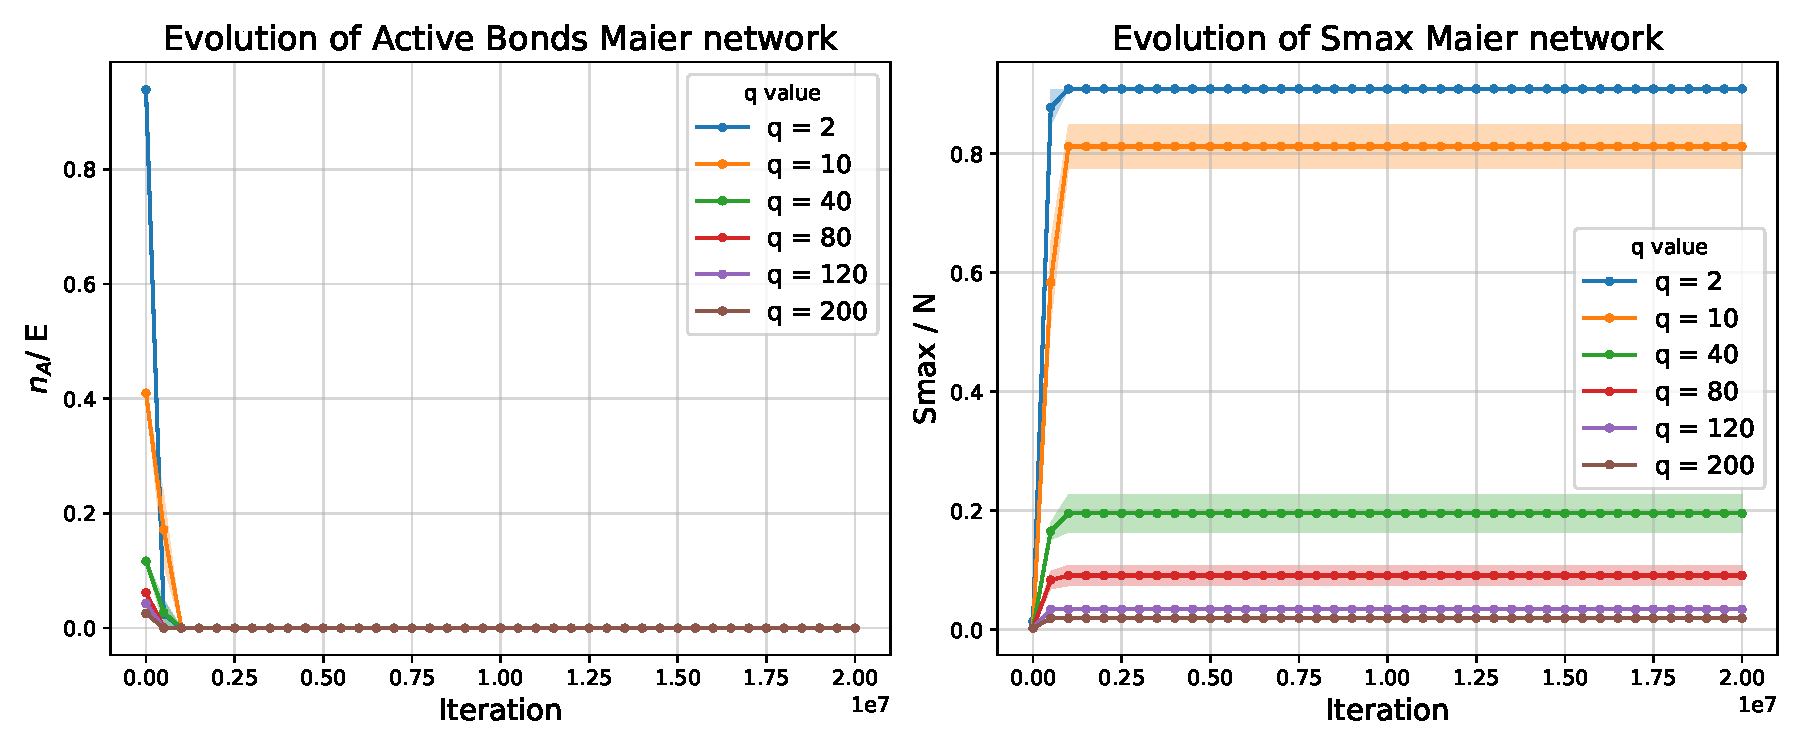
\includegraphics[width=0.9\linewidth]{task30_plots/evolution_plot_maier.pdf}
    \caption{Dynamics of the real network.}
    \label{fig:Maier_dynamics}
\end{figure}

As shown in Fig.~\ref{fig:Maier_dynamics}, the number of active bonds drops rapidly to zero, indicating that the system reaches an absorbing state almost immediately. This behavior is likely due to the fragmented structure of the network and the low initial overlap between neighboring nodes.

\begin{figure}[hbtp]
    \centering
    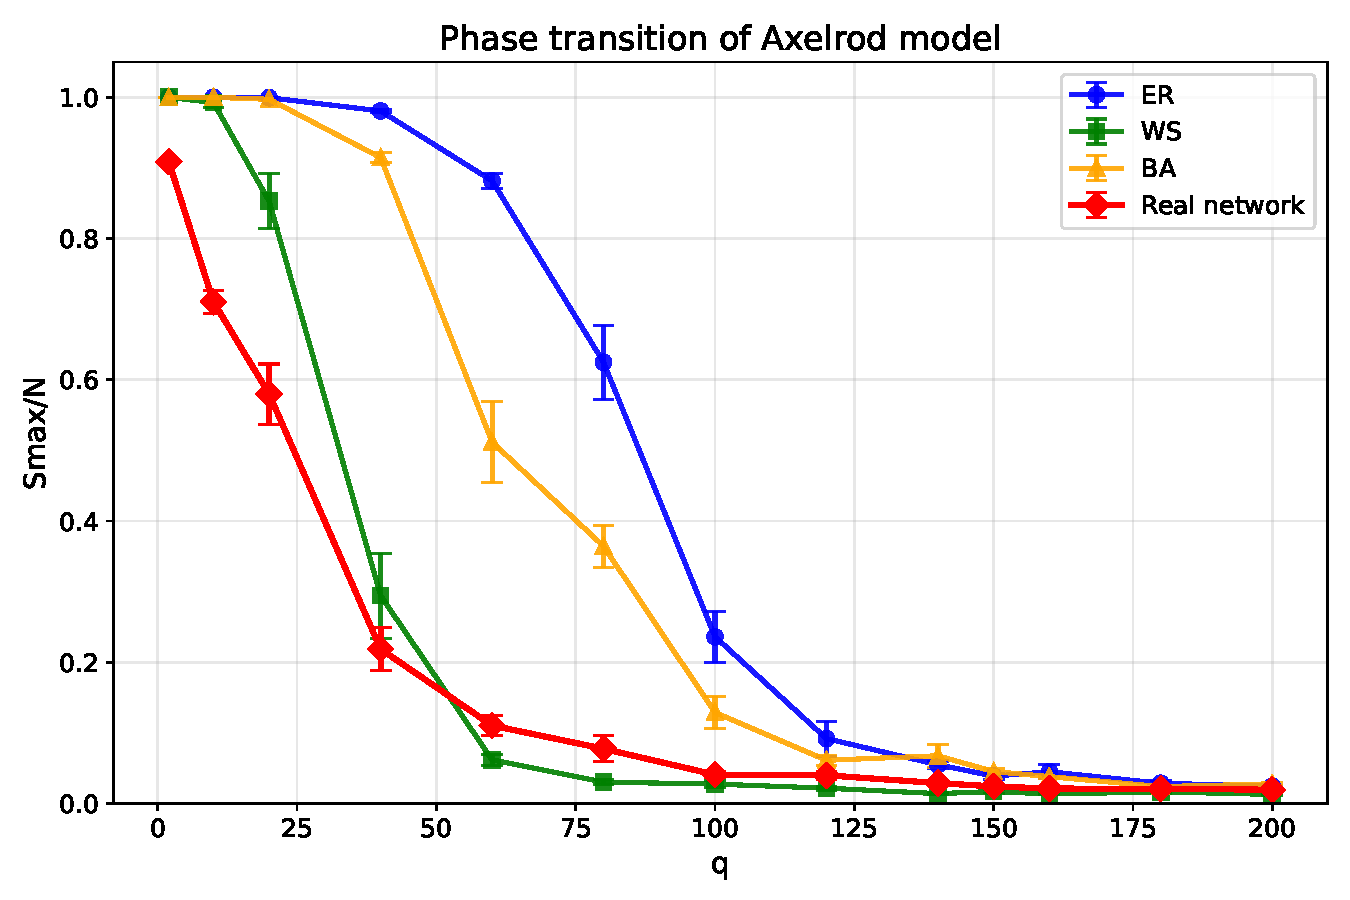
\includegraphics[width=0.75\linewidth]{task30_plots/real_network.pdf}
    \caption{Phase transition of the real network.}
    \label{fig:transition_real}
\end{figure}

From Fig. \ref{fig:transition_real}, we observe that the system behaves similarly to a small-world network, which is expected given its social network origin and the observed clustering and average path length. It is important to remark that this phase transition plot is qualitative, as the network contains fewer than 400 nodes and finite-size effects are dominant.
\newpage
\section{Subways II: results discussion}
Here a table with the main results is presented for visual and numerical clarity:

\begin{table}[h!]
\centering
\resizebox{\linewidth}{!}{
\begin{tabular}{|l|cccccc|}
\hline
\textbf{Network} & \textbf{Num nodes} & \textbf{Num edges} & \textbf{Assortativity} & \textbf{Avg short. path length} & \textbf{Avg degree} & \textbf{Avg betweenness} \\
\hline
Barcelona & 140 & 180 & 0.137 & 7.85 & 2.57 & 0.047 \\
Beijing   & 164 & 145 & 0.096 & 9.59 & 1.77 & 0.031 \\
Berlin    & 174 & 199 & 0.323 & 12.46 & 2.29 & 0.064 \\
Chicago   & 167 & 247 & 0.101 & 7.74 & 2.96 & 0.040 \\
HongKong  & 104 & 96  & 0.336 & 9.43 & 1.85 & 0.051 \\
London    & 333 & 408 & 0.297 & 11.31 & 2.45 & 0.020 \\
Madrid    & 306 & 250 & 0.204 & 10.55 & 1.63 & 0.015 \\
Mexico    & 148 & 164 & -0.110 & 11.01 & 2.22 & 0.068 \\
\hline
\end{tabular}
}
\caption{Network statistics for the analyzed subway networks.}
\label{tab:network_stats}
\end{table}

Network sizes range from Hong Kong's compact 104 nodes to London's extensive 333-station system. Assortativity values span from Mexico's negative correlation (-0.110) to Hong Kong's positive correlation (0.336), indicating fundamentally different connectivity patterns where some networks favor hub-to-hub connections while others distribute load through hub-to-peripheral designs. Chicago demonstrates optimal connectivity-efficiency balance with the highest average degree (2.96) and short path lengths (7.74), while Madrid's sparse connectivity (1.63 average degree) results in longer traversal times. Betweenness centrality variations highlight structural vulnerabilities, with Mexico's high value (0.068) suggesting critical node dependencies (as we can see in the betweenness distribution plot), whereas London's distributed architecture (0.020) provides greater robustness despite its scale. 


\section{Subways II: Average shortest path length vs degree assortativity}

To further examine the relationship between network topology and structural efficiency, we analyze the correlation between assortativity and average shortest path length across the subway networks, with node degree represented by color intensity and point size indicating network scale.

\begin{figure}[h!]
    \centering
    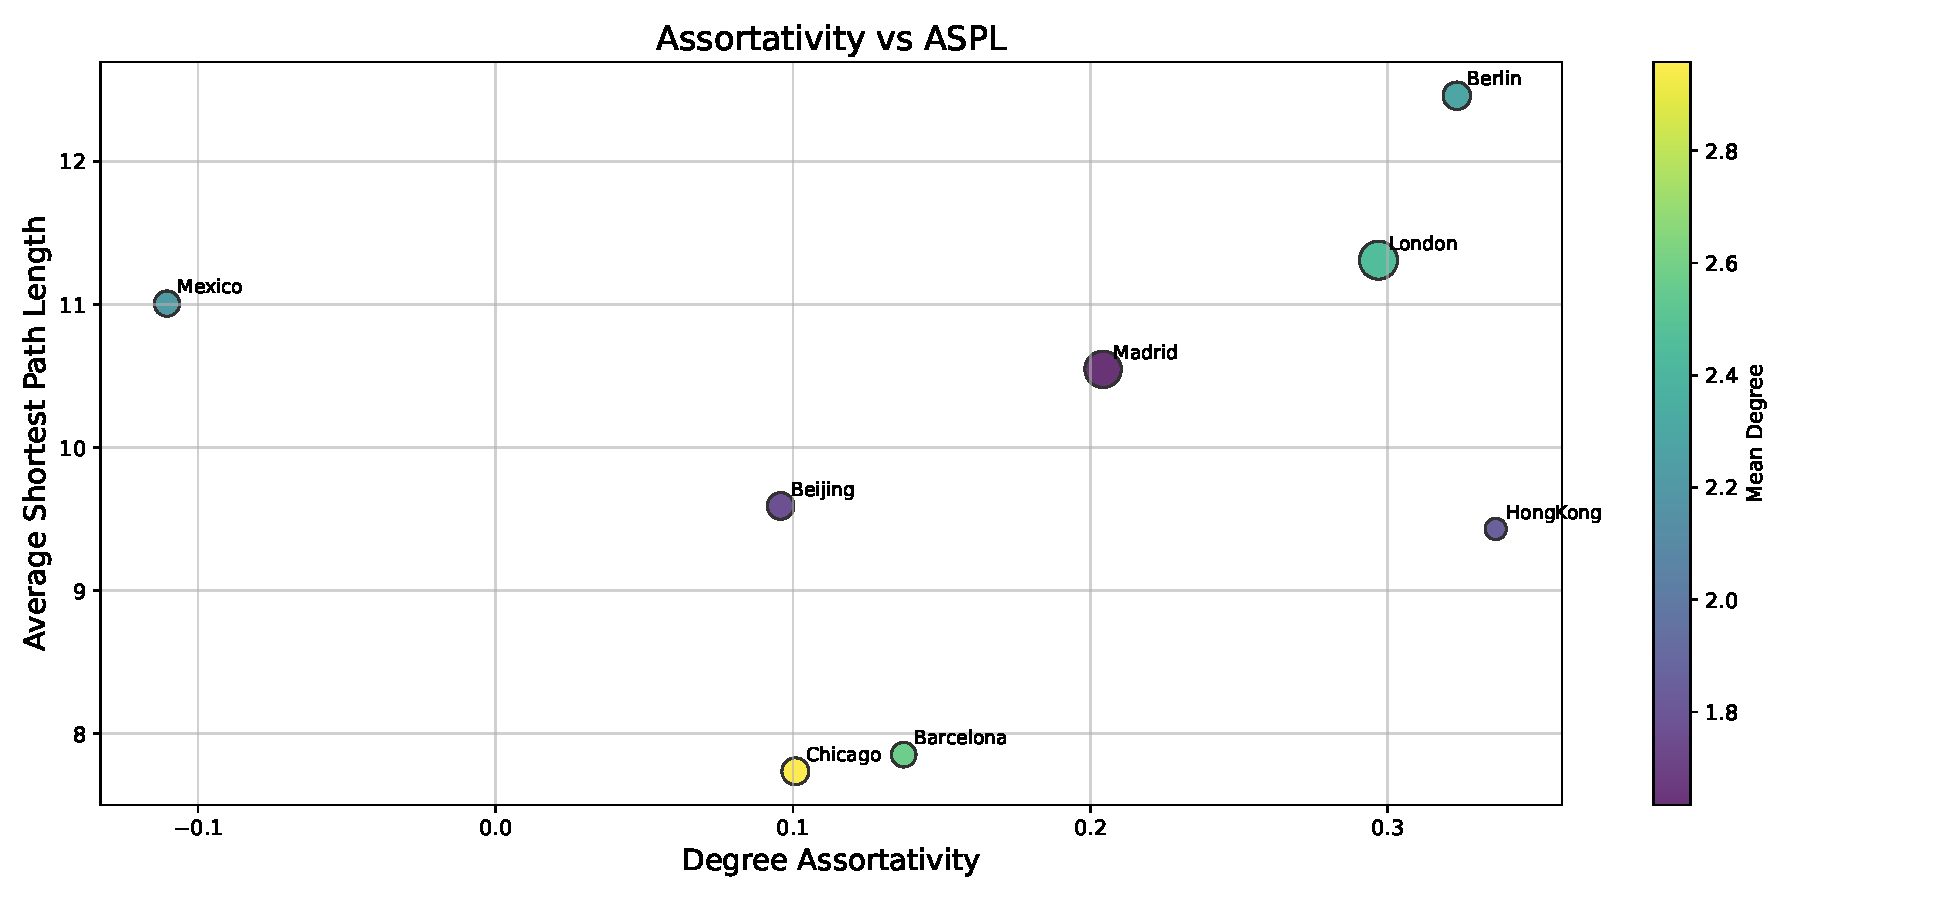
\includegraphics[width=0.8\linewidth]{task40_plots/correlation_plot.pdf}
    \caption{Correlation plot between average shortest path length and degree assortativity}
    \label{fig:aspl_vs_assort}
\end{figure}

The scatter plot seems to indicate a positive correlation between assortativity and average shortest path length, suggesting that networks where high-degree nodes preferentially connect to other high-degree nodes tend to have longer average traversal distances. This finding indicates that hierarchical, hub-centric designs may actually reduce overall network efficiency by forcing paths to route through central connection points rather than providing more direct routes. Networks with lower or negative assortativity, such as Mexico and Beijing, achieve shorter average path lengths despite having fewer highly connected nodes, suggesting that these systems prioritize direct connectivity over hierarchical organization. The point sizes reveal that this relationship holds across different network scales, from compact systems like Hong Kong to bigger networks like London. Interestingly, larger networks tend toward higher assortativity but maintain relatively moderate path lengths, indicating that scale allows for more sophisticated hierarchical designs without completely sacrificing efficiency.

While this analysis suggests a positive relationship between assortativity and average shortest path length, the small sample size (n=8) and potential confounding factors (geography, historical development) limit the statistical significance of this observation. 


